\documentclass[11pt]{article}

% ---------- Packages ----------
\usepackage[utf8]{inputenc}
\usepackage[margin=1in]{geometry}
\usepackage{graphicx}
\usepackage{amsmath}
\usepackage{amssymb}
\usepackage{listings}
\usepackage{xcolor}
\usepackage{caption}
\usepackage{subcaption}
\usepackage{float}
\usepackage{hyperref}

% ---------- Code listing style (for pasted code, optional) ----------
\definecolor{codegray}{rgb}{0.5,0.5,0.5}
\definecolor{codegreen}{rgb}{0,0.5,0}
\definecolor{codeblue}{rgb}{0.1,0.1,0.7}
\lstdefinestyle{py}{
    language=Python,
    basicstyle=\ttfamily\footnotesize,
    keywordstyle=\color{codeblue},
    commentstyle=\color{codegray}\itshape,
    stringstyle=\color{codegreen},
    numbers=none,
    breaklines=true,
    frame=single,
    rulecolor=\color{codegray},
    backgroundcolor=\color{gray!8},
    framesep=8pt,
    aboveskip=12pt,
    belowskip=12pt,
    showstringspaces=false,
    tabsize=4
}

\title{Homework Report}
\author{}
\date{}

\begin{document}
\maketitle

%==================================================================
\section{Problem 2.1: Sphere Tracing}
%==================================================================

\subsection{Code}

\noindent\textbf{Part A: Camera rays.}
\begin{lstlisting}[style=py]
def camera_param_to_rays(c2w, intrinsics, H=128, W=128):
    device = c2w.device
    c2w = c2w.to(torch.float32)
    intrinsics = intrinsics.to(torch.float32)
    fx, fy, cx, cy = intrinsics[0], intrinsics[1], intrinsics[2], intrinsics[3]

    # 1. Pixel grid: i indexes rows (y), j indexes columns (x)
    i, j = torch.meshgrid(
        torch.arange(H, device=device, dtype=torch.float32),
        torch.arange(W, device=device, dtype=torch.float32),
        indexing="ij",
    )
    x = j + 0.5  # shift to pixel centers
    y = i + 0.5

    # 2. Pixel -> camera coordinates
    X_cam = (x - cx) / fx
    Y_cam = (y - cy) / fy
    Z_cam = torch.ones_like(X_cam)
    dirs_cam = torch.stack([X_cam, Y_cam, Z_cam], dim=-1)  # [H, W, 3]

    # 3. Camera -> world (rotate by the rotation block of c2w)
    R = c2w[:3, :3]
    ray_directions = dirs_cam @ R.T  # [H, W, 3]

    # Normalize directions to unit length
    ray_directions = ray_directions / ray_directions.norm(dim=-1, keepdim=True)

    # Origins = camera position in world, broadcast to every pixel
    ray_origins = c2w[:3, 3].expand(H, W, 3).contiguous()

    return ray_origins, ray_directions
\end{lstlisting}

\noindent\textbf{Part B: Sphere tracing.}
\begin{lstlisting}[style=py]
def sphere_tracing(ray_origins, ray_directions, model,
                   t_near=0.0, t_far=3.0, max_iter=256, epsilon=1e-4):
    device = ray_origins.device
    H, W, _ = ray_origins.shape

    # Initialize output
    image = torch.zeros(H, W, 3, device=device)

    # 1. Initialize per-ray distance t and a hit mask
    t = torch.full((H, W), float(t_near), device=device)
    hit_mask = torch.zeros(H, W, dtype=torch.bool, device=device)

    # 2. March along the rays
    for _ in range(max_iter):
        # Current sample points along each ray
        points = ray_origins + t.unsqueeze(-1) * ray_directions  # [H, W, 3]

        # Query the implicit model (batched over all rays)
        sdf, color = model(points.reshape(-1, 3))
        sdf = sdf.reshape(H, W)
        color = color.reshape(H, W, 3)

        # Rays that hit the surface this step (and are still within range)
        newly_hit = (sdf < epsilon) & (~hit_mask) & (t <= t_far)

        # Record the surface color for newly-hit rays
        image[newly_hit] = color[newly_hit]
        hit_mask |= newly_hit

        # Advance only the rays that have not hit yet (0.5 relaxation factor)
        t = torch.where(hit_mask, t, t + 0.5 * sdf)

        # Early exit when everything has hit or marched past the far plane
        if hit_mask.all() or (t > t_far).all():
            break

    return image
\end{lstlisting}

\subsection{Rendered Result}
\begin{figure}[H]
    \centering
    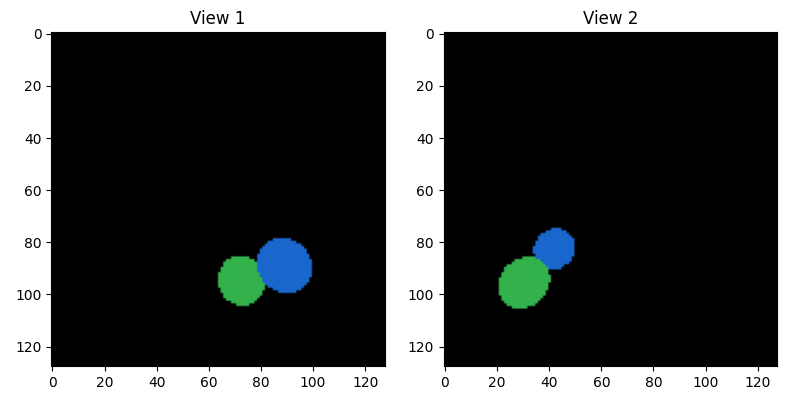
\includegraphics[width=0.9\linewidth]{images/sphere_tracing.png}
    \label{fig:sphere_tracing}
\end{figure}

%==================================================================
\section{Differentiable Volume Rendering}
%==================================================================

\subsection{Code}

\noindent\textbf{Part A: Camera rays.} Attached in 1A.

\medskip
\noindent\textbf{Part B: Ray marching.}
\begin{lstlisting}[style=py]
def sample_points_on_rays(ray_origins, ray_directions,
                          num_samples=64, t_near=0.0, t_far=3.0):
    device = ray_origins.device

    # 1. Uniformly spaced distances along every ray
    ts = torch.linspace(t_near, t_far, num_samples, device=device)  # [num_samples]

    # 2. point = origin + t * direction, broadcast over the sample dimension
    points = (
        ray_origins[..., None, :]
        + ts[None, None, :, None] * ray_directions[..., None, :]
    )  # [H, W, num_samples, 3]

    return points, ts
\end{lstlisting}

\noindent\textbf{Part C: Volumetric rendering.}
\begin{lstlisting}[style=py]
def volume_rendering(densities, colors, deltas):
    # Broadcast deltas over [H, W, N, 1]
    deltas = deltas.view(1, 1, -1, 1)

    # alpha_i = 1 - exp(-sigma_i * delta_i)
    alpha = 1.0 - torch.exp(-densities * deltas)  # [H, W, N, 1]

    # Accumulated transmittance T_i = prod_{j < i} (1 - alpha_j)  (exclusive)
    ones = torch.ones_like(alpha[:, :, :1, :])
    T = torch.cumprod(
        torch.cat([ones, 1.0 - alpha + 1e-10], dim=2), dim=2
    )[:, :, :-1, :]

    # Per-sample weights and final color C = sum_i T_i * alpha_i * c_i
    weights = T * alpha  # [H, W, N, 1]
    image = (weights * colors).sum(dim=2)  # [H, W, 3]

    return image
\end{lstlisting}

\subsection{Rendered Result}
\begin{figure}[H]
    \centering
    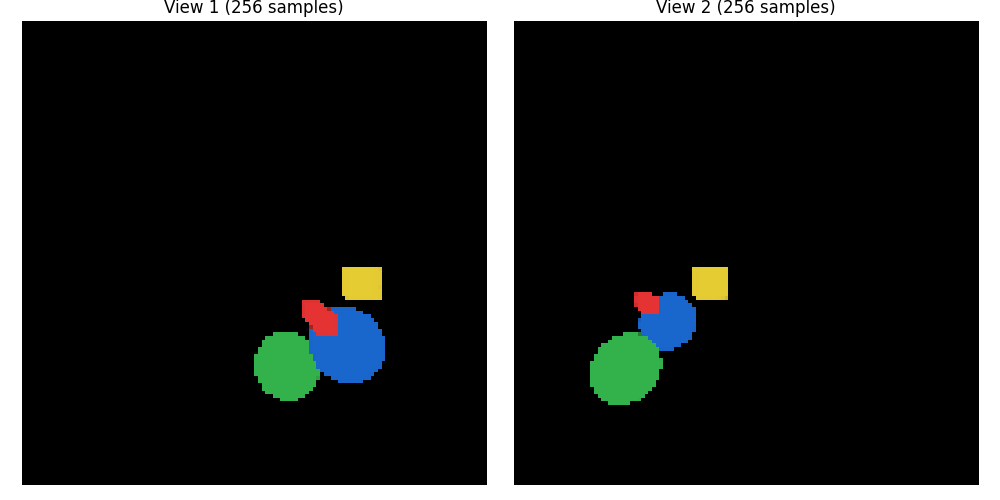
\includegraphics[width=0.9\linewidth]{images/volume_rendering.png}
    \label{fig:volume_rendering}
\end{figure}

%==================================================================
\subsection{Why is volume rendering preferred over sphere tracing?}
%==================================================================

Not everything has a strict surface. Sphere tracing expects the world to be made of solid objects.  But if you try to render smoke, hair, or fire, there's no real 'surface' to hit. Volume rendering just uses a density field, so it naturally handles all the fluffy and transparent stuff that SDFs struggle with.


%==================================================================
\section{Extra Challenge}
%==================================================================

\subsection{Effect of the number of samples}
% -------- Place renders with different sample counts here --------
\begin{figure}[H]
    \centering
    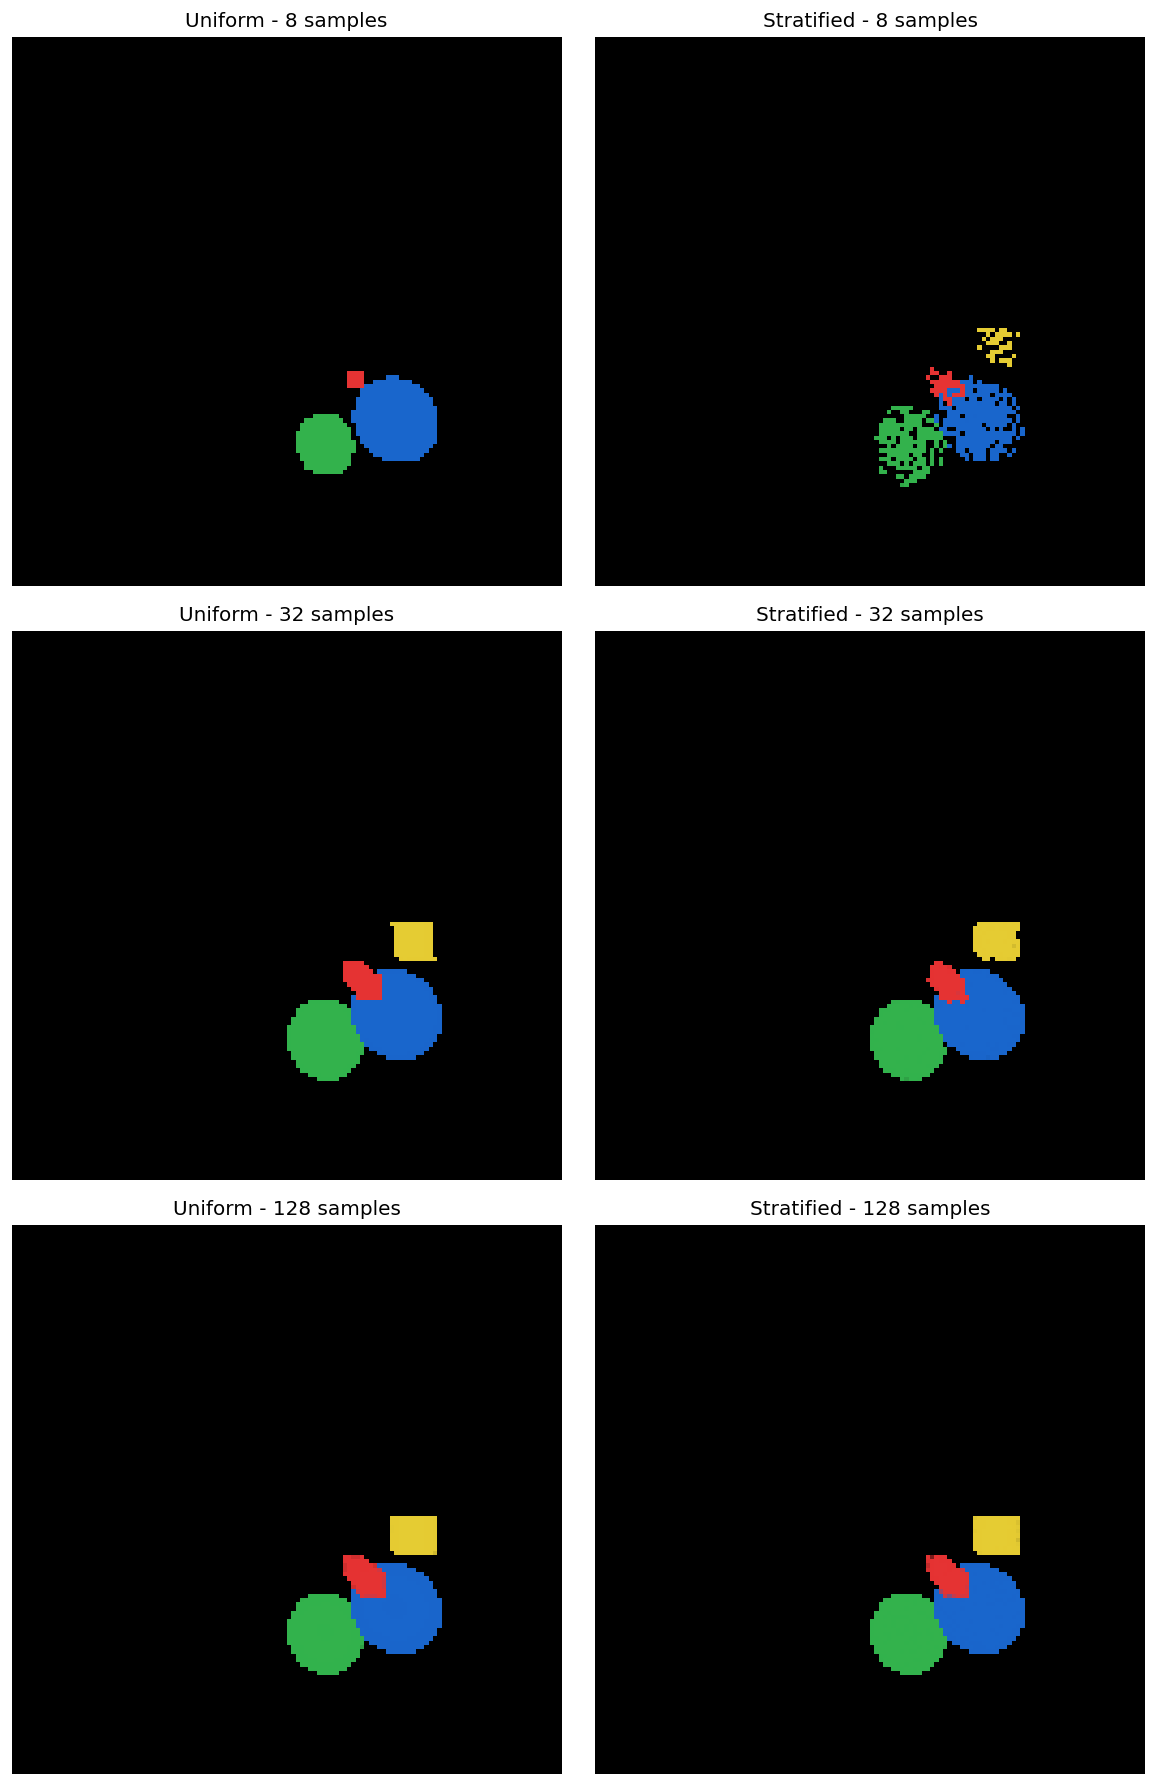
\includegraphics[width=0.9\linewidth]{images/extra_challenge_comparison.png}
    \caption{Effect of changing the number of samples along each ray
    (e.g.\ 16 / 64 / 256 samples).}
    \label{fig:samples}
\end{figure}


%==================================================================
\section{Problem 3: Playing with a NeRF}
%==================================================================

\subsection{Positional Encoding of NeRF}

\noindent\textbf{Code (filled-in lines).}
\begin{lstlisting}[style=py]
# Create a tensor of frequencies.
# Lowest frequency is 2*pi, each subsequent frequency doubles: omega_k = 2*pi * 2**k
freq_bands = 2.0 * torch.pi * (
    2.0 ** torch.arange(
        self.num_octaves, device=samples.device, dtype=samples.dtype
    )
)

# Fill the tensor with sine and cosine embedded values.
for i, freq in enumerate(freq_bands):
    embedded_samples[..., i :: 2 * self.num_octaves] = torch.sin(samples * freq)
    embedded_samples[..., i + self.num_octaves :: 2 * self.num_octaves] = (
        torch.cos(samples * freq)
    )
\end{lstlisting}

% --- Optional: replace the listing above with a screenshot of your code ---
% \begin{figure}[h]
%     \centering
%     \includegraphics[width=\linewidth]{images/code_positional_encoding.png}
%     \caption{Filled-in \texttt{PositionalEncoding.forward}.}
% \end{figure}

\paragraph{Test result.} Running \texttt{python -m tests.test\_positional\_encoding} passes.
\begin{figure}[H]
    \centering
    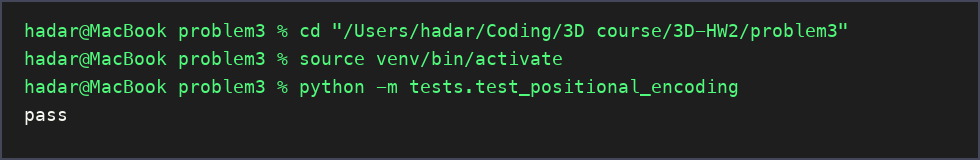
\includegraphics[width=0.85\linewidth]{images/pe_test_pass.png}
    \caption{Output of the positional-encoding unit test.}
    \label{fig:pe_test}
\end{figure}

\subsection{NeRF Forward Pass}

The volumetric rendering in \texttt{src/nerf.py} was already mostly implemented; only the final
compositing call had to be filled in. The full \texttt{forward} method is shown below. After
generating midpoint samples along each ray, evaluating the field, and computing the per-segment
$\alpha$ values, the ray color is obtained by alpha-compositing the colors with their $\alpha$
values (assuming a black background). The filled-in line is marked in the listing.

\begin{lstlisting}[style=py]
def forward(
    self,
    origins: Float[Tensor, "batch 3"],
    directions: Float[Tensor, "batch 3"],
    near: float,
    far: float,
) -> Float[Tensor, "batch 3"]:
    num_samples = self.cfg.num_samples
    # 1. Generate sample locations along the rays
    sample_locations, boundaries = self.generate_samples(
        origins, directions, near, far, num_samples
    )

    # 2. Evaluate the neural field at the sample locations
    field_outputs = self.field(sample_locations.reshape(-1, 3)).reshape(
        origins.size(0), num_samples, -1
    )

    colors = field_outputs[..., :3]  # RGB colors
    densities = field_outputs[..., 3]  # Volumetric densities

    # 3. Compute the alpha values
    alphas = self.compute_alpha_values(densities, boundaries)

    # 4. Composite the alpha values and colors (filled in)
    radiance = self.alpha_composite(alphas, colors)

    return radiance
\end{lstlisting}

\subsection{Question: Difference from the Original NeRF Paper}

The rendering model in this assignment differs from the original NeRF paper in (at least)
the following ways (the hint points at \emph{rendering} and \emph{ray sampling}):

\begin{itemize}
    \item \textbf{No view-direction dependence (rendering).} Our neural field maps a 3D
    \emph{position} $\mathbf{x}=(x,y,z)$ directly to an RGB color and a density. The original
    NeRF additionally conditions the color on the \emph{viewing direction} $\mathbf{d}$
    (a 5D input $(\mathbf{x},\mathbf{d})$), which lets it model view-dependent effects such as
    specular highlights and reflections. Our color is purely a function of position, so it
    cannot represent such effects.

    \item \textbf{Deterministic, single-scale ray sampling (ray sampling).} We split each ray
    into equally spaced segments and always query the fixed \emph{midpoints} of those segments
    (see \texttt{generate\_samples}). The original NeRF instead uses \emph{stratified} sampling
    (a random jitter within each bin during training) and a \emph{hierarchical} coarse-to-fine
    scheme with two networks, where a second ``fine'' network is sampled more densely around
    regions of high density predicted by the ``coarse'' network. Our implementation uses a
    single network with no random jitter and no hierarchical resampling.
\end{itemize}

\noindent\textit{(Either of the two points above is a sufficient answer to the question.)}

\subsection{Final Rendering (\texttt{outputs/spin})}

The model was trained with \texttt{python -m scripts.train\_nerf}. Below are final views from
the \texttt{outputs/spin} folder. The 3D structure of the \texttt{lego} scene is perceivable
even though the result is somewhat blurred.

\begin{figure}[H]
    \centering
    \begin{subfigure}{0.32\linewidth}
        \centering
        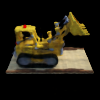
\includegraphics[width=\linewidth]{images/spin_1.png}
        \caption{View 1 ($0^{\circ}$ azimuth).}
    \end{subfigure}
    \hfill
    \begin{subfigure}{0.32\linewidth}
        \centering
        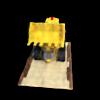
\includegraphics[width=\linewidth]{images/spin_2.png}
        \caption{View 2 ($\approx 96^{\circ}$ azimuth).}
    \end{subfigure}
    \hfill
    \begin{subfigure}{0.32\linewidth}
        \centering
        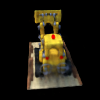
\includegraphics[width=\linewidth]{images/spin_3.png}
        \caption{View 3 ($\approx 264^{\circ}$ azimuth).}
    \end{subfigure}
    \caption{Final renderings from the \texttt{outputs/spin} folder after training (30-step camera orbit).}
    \label{fig:spin}
\end{figure}

\noindent\textbf{Training configuration.} The model was trained on an Apple M2 MacBook using
MPS (Metal GPU acceleration) with the default settings in \texttt{config/train\_nerf.yaml} and
\texttt{config/field/mlp.yaml}: 8192 iterations, learning rate $10^{-3}$, batch size 512,
128 samples per ray, 4 hidden MLP layers with hidden dimension 256, and 6 positional-encoding
octaves. Training took approximately 14 minutes end-to-end on MPS.

\end{document}
